\chapter{Image processing}
\label{chap-images}
\chapteroverview{A digital image is an array of numbers, so changing an image means computing with those numbers. This chapter develops simple methods for storing images, removing noise, detecting edges and manipulating colors. Each example connects a visible effect with an explicit formula and explains the information that the operation preserves or loses.}

\section{Pixels and grayscale values}
A grayscale image with $n$ rows and $p$ columns contains $np$ \emph{pixels}. In the eight-bit representation considered here, each pixel stores an integer between $0$ and $255=2^8-1$. Zero is displayed as black, 255 as white, and the intermediate values as shades of gray. Other bit depths and floating-point representations are also used.

The flower in Figure~\ref{fig-section1-original-zoom} has $256\times256=65\,536$ pixels. The enlargement shows a $5\times5$ patch: each displayed shade corresponds to one of the numbers in the array. A photograph may contain millions of pixels, but the same representation applies.
\myfigure{\imageL{section1-original-zoom}}
{An image and a magnified $5\times5$ patch of pixel values.}{fig-section1-original-zoom}

\section{Storing an image}
\subsection{Binary representation and storage units}
An integer is represented in binary by decomposing it into powers of two. For example,
\[
 179=2^7+2^5+2^4+2^1+2^0
    =\underbrace{(10110011)_2}_{\text{binary representation}}.
\]
Reading from $2^7$ down to $2^0$, a bit is one when the corresponding power occurs and zero otherwise. Eight bits suffice for every integer from 0 to 255.

An uncompressed eight-bit grayscale image therefore requires $8np$ bits, or $np$ \emph{bytes}, for its pixel values. The $256\times256$ flower uses
\[
 256\times256\times8=524\,288\ \text{bits}
       =65\,536\ \text{bytes}.
\]
This is $65.536$ kB in decimal units, or $64$ KiB in binary units: $1$ kB is $1000$ bytes, whereas $1$ KiB is $1024$ bytes. For comparison, a $240\times240$ image would require $57\,600$ bytes, or $56.25$ KiB. File headers and metadata add to these payload sizes.

\subsection{Subsampling}
Reducing the number of pixels reduces storage. Keeping every fourth row and every fourth column divides the pixel count by $4^2=16$, when both dimensions are divisible by four. Figure~\ref{fig-section2-subsample} shows increasingly coarse grids.
\myfigure{\imageTri{section2-subsample-4}{section2-subsample-8}{section2-subsample-16}
{One row/column in 4}{One row/column in 8}{One row/column in 16}}
{Subsampling on successively coarser grids.}{fig-section2-subsample}

Discarding rows and columns can lose fine detail and create false patterns, an effect called \emph{aliasing}. A practical resizing method usually smooths the image before reducing its sampling rate. The next chapter explains the mathematical reason for this precaution.

\subsection{Quantization}
Storage can also be reduced by using fewer possible values per pixel. To retain four levels, replace an input value $a\in\{0,\ldots,255\}$ by
\[
 q(a)=\left\lfloor\frac a{64}\right\rfloor\in\{0,1,2,3\}.
\]
Thus $0$--$63$ map to $0$, $64$--$127$ to $1$, $128$--$191$ to $2$, and $192$--$255$ to $3$. When displayed on a scale from black to white, these indices correspond respectively to black, dark gray, light gray and white; they can be rendered using the values $85q(a)$.

Four indices require two bits, rather than eight, giving a factor-four saving if the indices are packed into the file. Merely storing the indices in eight-bit containers would not achieve that saving. Figure~\ref{fig-section3-quantize} compares four and sixteen levels.
\myfigure{\imageDuo{section3-quantize-4}{section3-quantize-16}{4 gray levels}{16 gray levels}}
{Quantization with two different numbers of levels.}{fig-section3-quantize}

Quantization is generally irreversible: many original values share the same index. Lossless compression, by contrast, preserves every input value while exploiting redundancy in its representation. JPEG 2000 uses wavelets and offers both lossless and lossy modes; it is one example of a codec, not a universally best choice for every image and criterion.\footnote{\url{https://jpeg.org/jpeg2000/}}

\section{Removing noise}
\subsection{Local averaging}
Noise produces unwanted fluctuations in pixel values. It is particularly visible in low-light photographs, although its distribution depends on the sensor and acquisition process. A simple denoising method replaces each pixel by the mean of a surrounding window.

For the $3\times3$ neighborhood in Figure~\ref{fig-section5-moyenne-numbers}, replace the central value $a$ by
\[
 \frac{a+b+c+d+e+f+g+h+i}{9}.
\]
The displayed values give
\[
 \frac{190+192+79+54+47+153+203+189+166}{9}
       =\frac{1273}{9}\simeq141.44.
\]
\myfigure{\imageM{section5-moyenne-numbers}}
{A $3\times3$ neighborhood used for local averaging and median filtering.}{fig-section5-moyenne-numbers}

All averages must be computed from the same input image. Updating pixels in place and then reusing those updated values defines a different filter. At the image boundary, one must also choose a rule, such as reflecting the image or restricting and renormalizing the window.

Why does averaging help? If a locally constant signal is corrupted by independent, zero-mean noise of variance $\sigma^2$, the average of $m$ pixels has noise variance $\sigma^2/m$. Near an edge, however, the underlying signal is not constant: averaging mixes distinct regions and introduces blur. A larger window trades more noise reduction for more loss of detail.
\myfigure{\begin{tabular}{@{}c@{\hspace{2mm}}c@{\hspace{2mm}}c@{\hspace{2mm}}c@{}}
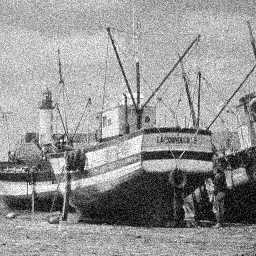
\includegraphics[width=.23\linewidth]{section5-noisy}&
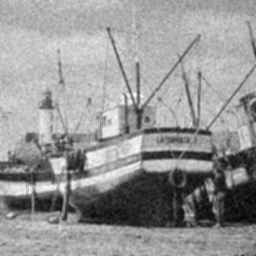
\includegraphics[width=.23\linewidth]{section5-moyenne-1}&
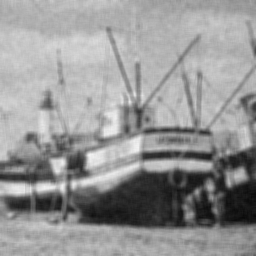
\includegraphics[width=.23\linewidth]{section5-moyenne-2}&
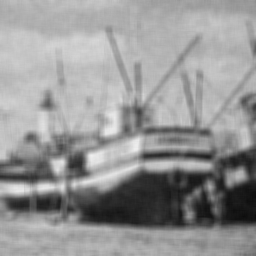
\includegraphics[width=.23\linewidth]{section5-moyenne-3}\\
Noisy image&$3\times3$ mean&$5\times5$ mean&$7\times7$ mean
\end{tabular}}{Local averaging reduces noise but blurs edges as the window grows.}{fig-section5-moyenne}

\subsection{Local median}
The \emph{median} of an odd number of values is the middle value after sorting. The nine values above, in increasing order, are
\[
 47,54,79,153,166,189,190,192,203,
\]
so their median is $166$. A median filter replaces each pixel by the median of its input neighborhood.

The median is resistant to isolated extreme values and often preserves sharp transitions better than the mean. It is particularly useful for impulse noise, but it is not uniformly better for every noise model or image. Large windows can erase thin objects and small details. Figure~\ref{fig-section6-mediane} illustrates this tradeoff.
\myfigure{\begin{tabular}{@{}c@{\hspace{2mm}}c@{\hspace{2mm}}c@{\hspace{2mm}}c@{}}
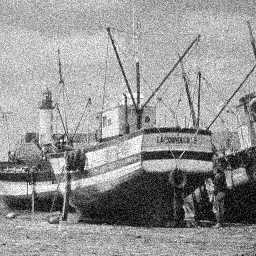
\includegraphics[width=.23\linewidth]{section5-noisy}&
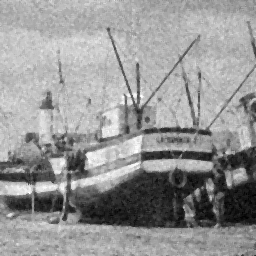
\includegraphics[width=.23\linewidth]{section6-mediane-1}&
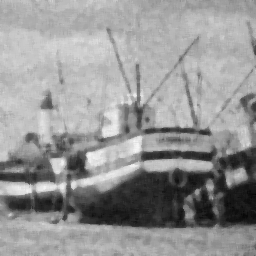
\includegraphics[width=.23\linewidth]{section6-mediane-2}&
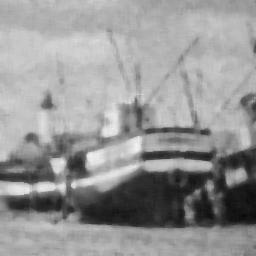
\includegraphics[width=.23\linewidth]{section6-mediane-3}\\
Noisy image&$3\times3$ median&$5\times5$ median&$7\times7$ median
\end{tabular}}{Median filtering with increasing window size.}{fig-section6-mediane}

\section{Detecting edges}
Edges are locations where pixel values change rapidly, for instance at a boundary between a dark object and a bright background. A simple detector compares the neighbors on opposite sides of a pixel.
\myfigure{\imageM{section7-contours-numbers}}
{The central pixel $a$ and its left, upper, right and lower neighbors $b,c,d,e$.}{fig-section7-contours-numbers}

With the arrangement of Figure~\ref{fig-section7-contours-numbers}, define
\[
 \ell=\sqrt{(b-d)^2+(c-e)^2}.
\]
For unit pixel spacing, $\ell/2$ is the magnitude of the gradient estimated by centered differences. The values in the figure yield
\[
 \ell=\sqrt{(192-153)^2+(54-189)^2}
      =\sqrt{19\,746}\simeq140.52.
\]
We have $\ell=0$ exactly when $b=d$ and $c=e$. This does not imply that all five values are equal: the detector can miss some fine oscillations. A large value indicates a strong local variation, which may come from an object boundary, texture or noise.

For display, the value is clipped to $\min(\ell,255)$ and rounded. The minimum is needed because $\ell$ can exceed 255. Figure~\ref{fig-section7-contours} displays large responses in white. Denoising before differentiation can help because differences also amplify noise.
\myfigure{\imageDuo{section7-image}{section7-contours}{Original image}{Edge response $\ell$}}
{Edge detection by differences between opposite neighbors.}{fig-section7-contours}

\section{Color images}
\subsection{RGB channels and additive color}
An RGB image has three channels, representing red, green and blue. They are separate arrays, but are generally \emph{not statistically independent}. In an eight-bit representation, a pixel is a triplet $(r,g,b)\in\{0,\ldots,255\}^3$ and requires 24 bits before compression.

The values $(255,0,0)$, $(0,255,0)$ and $(0,0,255)$ display red, green and blue respectively. Combining emitted light follows \emph{additive} color mixing: red plus green, $(255,255,0)$, gives yellow; red plus blue, $(255,0,255)$, gives magenta. White is $(255,255,255)$ and black is $(0,0,0)$.
\myfigure{\imageDuo{section8-image}{section8-luminance}{Color image}{Mean-channel grayscale}}
{A color image and a grayscale representation.}{fig-luminance}
\myfigure{\imageTri{section8-rouge}{section8-vert}{section8-bleu}{Red channel}{Green channel}{Blue channel}}
{The three RGB channels, displayed in their corresponding colors.}{fig-canaux-coul}
\myfigure{\imageDuo{section8-synthese-additive}{section8-synthese-soustractive}{Additive mixing}{Subtractive mixing}}
{Idealized additive and subtractive color mixing.}{fig-section8-synthese}

\subsection{CMY channels and subtractive color}
An idealized complementary representation uses cyan, magenta and yellow:
\[
 c=255-r,\qquad m=255-g,\qquad y=255-b.
\]
For example, blue $(r,g,b)=(0,0,255)$ corresponds to $(c,m,y)=(255,255,0)$. These variables describe the \emph{subtractive} action of ideal pigments on white light: cyan absorbs red, magenta absorbs green, and yellow absorbs blue.
\myfigure{\imageTri{section8-cyan}{section8-magenta}{section8-jaune}{Cyan channel}{Magenta channel}{Yellow channel}}
{The complementary CMY channels, shown against white backgrounds.}{fig-canaux-cmj}

Real printers use device-dependent color conversions, usually with an additional black channel (CMYK). A screen still emits RGB light, so CMY data must be converted for display. Neither a fixed set of display primaries nor a fixed set of inks reproduces every visible color.

\section{Changing brightness and contrast}
\subsection{A grayscale intensity}
A simple way to obtain a grayscale image is to average the three channels:
\[
 a=\frac{r+g+b}{3}.
\]
This is the intensity used in the elementary examples here. It is not the physical \emph{luminance}, which weights linear-light components according to visual sensitivity. In particular, an arithmetic mean of encoded RGB values is not a calibrated measurement of emitted light.\footnote{For the definition of relative luminance in sRGB, see \url{https://www.w3.org/TR/WCAG22/\#dfn-relative-luminance}.}

\subsection{Pointwise changes in grayscale}
Replacing $a$ by $255-a$ exchanges black and white and produces a negative. To darken an image, use $a\mapsto a^2/255$; to brighten it, use $a\mapsto\sqrt{255a}$. Both maps preserve the interval $[0,255]$.
\myfigure{\imageTri{section4-negatif}{section4-square}{section4-sqrt}{Negative}{Square: darker}{Square root: brighter}}
{Three pointwise transformations of grayscale intensity.}{fig-section4-square}

The square and square-root maps are inverses as functions on the real interval. After rounding to integer pixel values, they need not undo one another exactly. Their common generalization is the power transformation
\[
 \widetilde a=255\left(\frac a{255}\right)^\gamma,
 \qquad \gamma>0,
\]
with $\widetilde a=0$ when $a=0$. For $0<a<255$, the image becomes brighter when $\gamma<1$ and darker when $\gamma>1$. The cases $\gamma=1/2$ and $\gamma=2$ give the square root and square, respectively; $\gamma=1$ leaves the values unchanged.

\subsection{A color transformation}
Applying unrelated changes to the three channels can alter colors strongly. One elementary alternative changes the mean intensity $a$ while keeping the residual $(r-a,g-a,b-a)$ fixed. Define
\[
 \begin{aligned}
 \widetilde r&=\operatorname{clip}(r+\widetilde a-a),\\
 \widetilde g&=\operatorname{clip}(g+\widetilde a-a),\\
 \widetilde b&=\operatorname{clip}(b+\widetilde a-a),
 \end{aligned}
 \qquad \operatorname{clip}(u)=\max(0,\min(255,u)).
\]
Without clipping, the new mean is $\widetilde a$ and the differences between channels are preserved. Clipping can change both properties, and this construction does not guarantee exact preservation of perceived hue or saturation. Values are rounded only after the computation.
\myfigure{\begin{tabular}{@{}c@{\hspace{1mm}}c@{\hspace{1mm}}c@{\hspace{1mm}}c@{\hspace{1mm}}c@{\hspace{1mm}}c@{}}
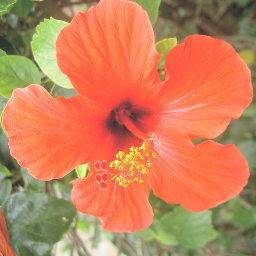
\includegraphics[width=.15\linewidth]{section4-constrast-1}&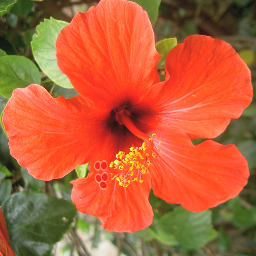
\includegraphics[width=.15\linewidth]{section4-constrast-2}&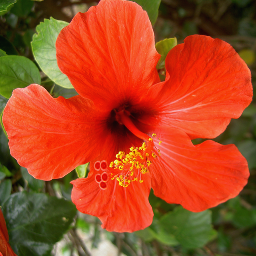
\includegraphics[width=.15\linewidth]{section4-constrast-3}&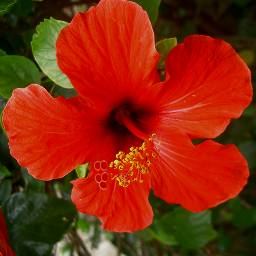
\includegraphics[width=.15\linewidth]{section4-constrast-4}&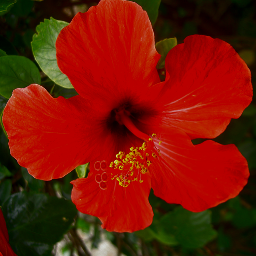
\includegraphics[width=.15\linewidth]{section4-constrast-5}&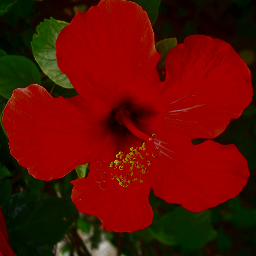
\includegraphics[width=.15\linewidth]{section4-constrast-6}\\
$\gamma=0.5$&$0.75$&$1$&$1.5$&$2$&$3$
\end{tabular}}{Changing a color image through a power transformation of its mean intensity.}{fig-contrast-color}

\section{Images as matrices}
\subsection{Transposition and rotation}
Write an image as a matrix $A=(a_{i,j})\in\mathbb{R}^{n\times p}$. Rows are indexed from top to bottom by $1\leq i\leq n$ and columns from left to right by $1\leq j\leq p$. Its transpose $B=A^{\mathsf T}\in\mathbb{R}^{p\times n}$ satisfies
\[
 b_{j,i}=a_{i,j}.
\]
It exchanges the two coordinate directions and reflects the image across the diagonal direction. A clockwise quarter-turn produces another $p\times n$ matrix $C$ given by
\[
 c_{j,i}=a_{n-i+1,j},\qquad 1\leq j\leq p,\quad1\leq i\leq n.
\]
Equivalently, the original pixel $(i,j)$ moves to $(j,n-i+1)$. These operations permute pixel values and therefore lose no information. Apply the same permutation to all channels of a color image.
\myfigure{\imageTri{section10-original}{section10-transpose}{section10-rotation}{$A$}{$A^{\mathsf T}$}{Clockwise rotation}}
{Transposition and rotation by a quarter-turn.}{fig-geometric}

\subsection{A crossfade between two images}
For images $A$ and $B$ of the same dimensions and channel format, define
\[
 C_t=(1-t)A+tB,\qquad 0\leq t\leq1.
\]
This formula is applied to each pixel and channel. The endpoints are $C_0=A$ and $C_1=B$; intermediate values produce a \emph{crossfade}. Because the weights are nonnegative and sum to one, values stay in $[0,255]$ before rounding. This blends colors at fixed locations; it does not move objects from one location to another.
\myfigure{\begin{tabular}{@{}c@{\hspace{1mm}}c@{\hspace{1mm}}c@{\hspace{1mm}}c@{\hspace{1mm}}c@{\hspace{1mm}}c@{}}
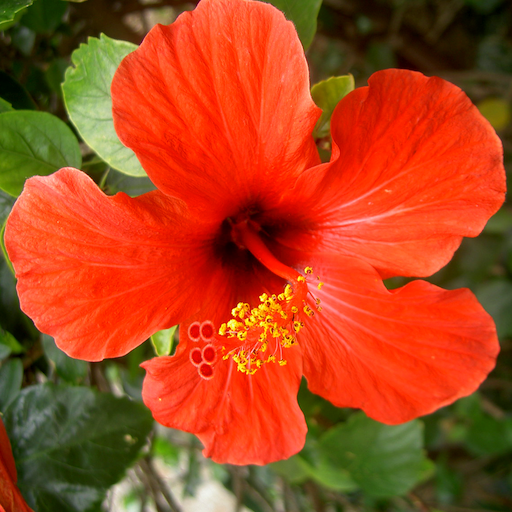
\includegraphics[width=.15\linewidth]{section11-interp-1}&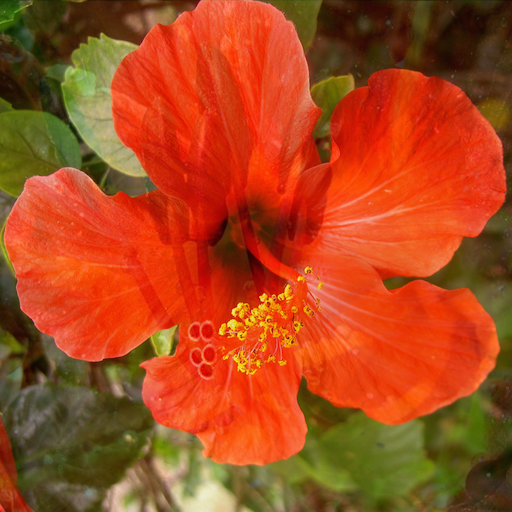
\includegraphics[width=.15\linewidth]{section11-interp-2}&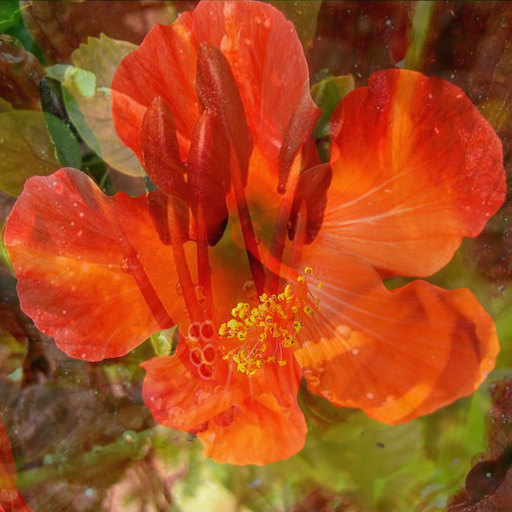
\includegraphics[width=.15\linewidth]{section11-interp-3}&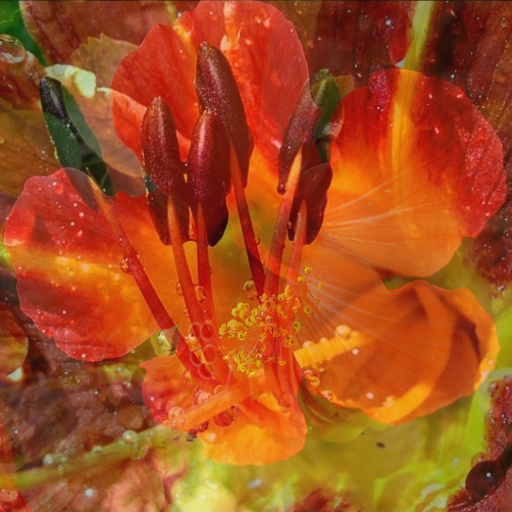
\includegraphics[width=.15\linewidth]{section11-interp-4}&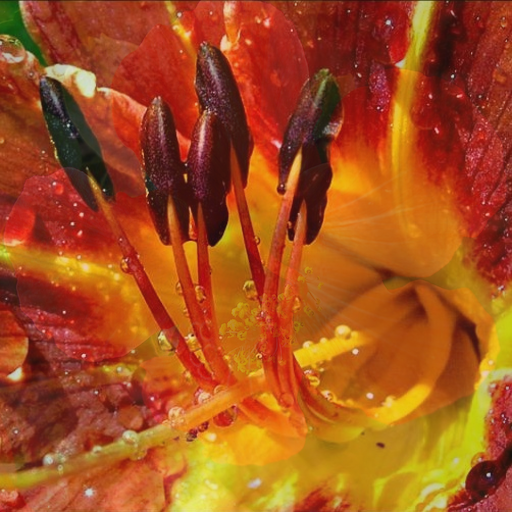
\includegraphics[width=.15\linewidth]{section11-interp-5}&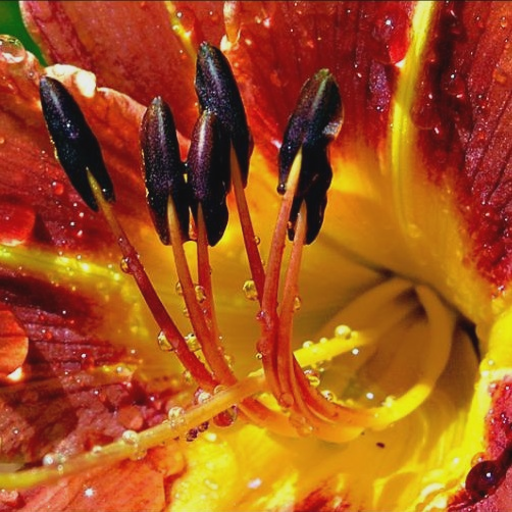
\includegraphics[width=.15\linewidth]{section11-interp-6}\\
$t=0$&$0.2$&$0.4$&$0.6$&$0.8$&$1$
\end{tabular}}{Linear interpolation from image $A$ to image $B$.}{fig-interp}

\paragraph*{Further reading.}
Reproducible examples are available in the \href{https://www.numerical-tours.com/}{Numerical Tours}~\cite{2011-peyre-cise}. This chapter draws in part on the author's article \emph{Le traitement numérique des images} in \emph{Images des mathématiques}.

\ifdefined\StandaloneChapter
\par\noindent\begin{minipage}{\linewidth}
\section*{Glossary}
\begin{multicols}{2}\small\raggedright
\begin{rs}
\gloss{Bit and byte}: a binary digit; a group of eight bits.
\gloss{Pixel}: one entry of an image array.
\gloss{Channel}: one component array of a multichannel image.
\gloss{Quantization}: replacing values by indices from a finite set.
\gloss{Noise}: unwanted fluctuations introduced by acquisition or processing.
\gloss{Mean}: the sum of values divided by their number.
\gloss{Median}: the central sorted value for an odd-sized set.
\gloss{Edge}: a rapid spatial change in image values.
\gloss{Blur}: a loss of sharp transitions and fine detail.
\gloss{Contrast}: differences between light and dark regions.
\gloss{Luminance}: a photometric quantity defined using visual sensitivity.
\gloss{Matrix}: a rectangular array $(a_{i,j})$.
\gloss{Resolution}: a term that may refer to pixel dimensions or to spatial resolving power; these are distinct notions.
\gloss{Crossfade}: a weighted average of two images at fixed pixel locations.
\end{rs}
\end{multicols}
\end{minipage}\par
\fi
